\documentclass{article}

% ===== Graphics =====
\usepackage{graphicx}
\usepackage{svg}
\graphicspath{{figures/}}
% Colors, table rule color, and caption styling
\usepackage[table]{xcolor}
\definecolor{darkgray}{HTML}{404040}
\arrayrulecolor{darkgray}
\usepackage{caption}
\captionsetup{labelfont={color=darkgray},textfont={color=darkgray}}
\usepackage{array}
\usepackage{tabularx}
\usepackage{threeparttable}
\usepackage{amsmath,amssymb}
\usepackage{tabularx}
\usepackage{dblfloatfix}
\usepackage{afterpage}

\usepackage[colorlinks=true,
linkcolor=blue,    % internal links (sections, equations, etc.)
citecolor=blue,    % citations in the bibliography
urlcolor=blue]     % URLs
{hyperref}



% Add these packages for better hyphenation control
\usepackage[english]{babel}  % Or german, french, etc. for language-specific rules
\usepackage{hyphenat}        % For additional hyphenation control
\hyphenation{}              % Add custom word break rules if needed





% --- required ---
\usepackage{xcolor}

% --- colors ---
\definecolor{usa_teal}{RGB}{0,255,255}
\definecolor{cn_orange}{RGB}{255,191,0}
\definecolor{eu_purple}{RGB}{255,0,255}
\definecolor{row_grey}{RGB}{220,220,220}

% ============================================================
%  Cluster label pills with hierarchical color intensities
% ============================================================

\usepackage[most]{tcolorbox}
\usepackage{xcolor}

% ---------- Define base colors ----------
\definecolor{clusterCS}{HTML}{9556CB} % Computer Science (purple)
\definecolor{clusterHS}{HTML}{619EFF} % Health Science (blue)
\definecolor{clusterSS}{HTML}{57DCCB} % Social Science (teal)
\definecolor{clusterNS}{HTML}{FFDD33} % Natural Science (yellow)
\definecolor{clusterE}{HTML}{FB7738}  % Engineering (orange)

% ---------- Shared pill style ----------
\tcbset{
	clusterstyle/.style={
		on line,
		boxrule=0pt,
		arc=2pt,
		top=1pt, bottom=1pt,
		left=3pt, right=3pt,
		boxsep=0pt,
		valign=center,
		colupper=black,
	}
}

% ============================================================
%                       MACRO LEVEL (20%)
% ============================================================
\newtcbox{\macroC}{clusterstyle, colback=clusterCS!20}
\newtcbox{\macroH}{clusterstyle, colback=clusterHS!20}
\newtcbox{\macroS}{clusterstyle, colback=clusterSS!20}
\newtcbox{\macroN}{clusterstyle, colback=clusterNS!20}
\newtcbox{\macroE}{clusterstyle, colback=clusterE!20}

% ============================================================
%                       MESO LEVEL (50%)
% ============================================================
\newtcbox{\mesoC}{clusterstyle, colback=clusterCS!50}
\newtcbox{\mesoH}{clusterstyle, colback=clusterHS!50}
\newtcbox{\mesoS}{clusterstyle, colback=clusterSS!50}
\newtcbox{\mesoN}{clusterstyle, colback=clusterNS!50}
\newtcbox{\mesoE}{clusterstyle, colback=clusterE!50}

% ============================================================
%                       MICRO LEVEL (80%)
% ============================================================
\newtcbox{\microC}{clusterstyle, colback=clusterCS!70}
\newtcbox{\microH}{clusterstyle, colback=clusterHS!70}
\newtcbox{\microS}{clusterstyle, colback=clusterSS!70}
\newtcbox{\microN}{clusterstyle, colback=clusterNS!70}
\newtcbox{\microE}{clusterstyle, colback=clusterE!70}





% 2) Make all badges the same size (inner width)
\newlength{\rankbadgewidth}
\setlength{\rankbadgewidth}{1.5em}  % fits 1-100 in bold

\newcommand{\badgebox}[2]{% #1=color, #2=rank text
	{\setlength{\fboxsep}{0.6pt}%
		\colorbox{#1}{\makebox[\rankbadgewidth][c]{\strut\textbf{#2}}}%
	}%
}


% --- EU-27 registry (silent; no text output) ---
\makeatletter
\def\EU@AT{}\def\EU@BE{}\def\EU@BG{}\def\EU@HR{}\def\EU@CY{}\def\EU@CZ{}\def\EU@DK{}\def\EU@EE{}%
\def\EU@FI{}\def\EU@FR{}\def\EU@DE{}\def\EU@GR{}\def\EU@HU{}\def\EU@IE{}\def\EU@IT{}\def\EU@LV{}%
\def\EU@LT{}\def\EU@LU{}\def\EU@MT{}\def\EU@NL{}\def\EU@PL{}\def\EU@PT{}\def\EU@RO{}\def\EU@SK{}%
\def\EU@SI{}\def\EU@ES{}\def\EU@SE{}%
% \IfEU{<ISO>}{<true>}{<false>}
\newcommand{\IfEU}[3]{%
	\edef\ISOtmp{#1}%
	\expandafter\@ifundefined\expandafter{EU@\ISOtmp}{#3}{#2}%
}
\makeatother

% --- choose badge color by ISO-2 (expects UPPERCASE ISO) ---
% Usage: \rankbadge{<rank>}{<ISO2>}
\newcommand{\rankbadge}[2]{%
	\begingroup
	\def\ISO{#2}%
	\def\US{US}\def\CN{CN}%
	\def\badgecol{row_grey}%
	\ifx\ISO\US \def\badgecol{usa_teal}\fi
	\ifx\ISO\CN \def\badgecol{cn_orange}\fi
	\IfEU{\ISO}{\def\badgecol{eu_purple}}{}%
	
	\def\HK{HK}\def\MO{MO}\def\TW{TW}%
	\ifx\ISO\HK \def\badgecol{cn_orange}\fi
	\ifx\ISO\MO \def\badgecol{cn_orange}\fi
	\ifx\ISO\TW \def\badgecol{cn_orange}\fi
	\makebox[2.4em][c]{\badgebox{\badgecol}{#1}}%
	\endgroup
}

% convenience alias used in the table
\newcommand{\rc}[2]{\rankbadge{#1}{#2}}



% Optional, for nicer rules and spacing
\usepackage{booktabs}



% ===== Colors =====
\usepackage{xcolor}
\definecolor{darkergray}{gray}{0.25}

% ===== Page layout =====
\usepackage[
a4paper,
top=2.5cm,
bottom=2.5cm,
left=1.5cm,
right=1.5cm,
columnsep=20pt
]{geometry}


% ===== Bibliography with biblatex =====
% NOTE: switched from numeric to author-date (Springer "Basic" style) for Scientometrics.
\usepackage[
backend=biber,
style=authoryear,
sorting=nyt,
maxcitenames=2,   % in-text: 3+ authors collapse to "First et al."
mincitenames=1,
maxbibnames=99    % reference list: keep ALL authors
]{biblatex}
\addbibresource{bibliography.bib} % <-- your .bib file location

% Make existing \cite calls render as parenthetical author-date, e.g. (Smith 2020).
\let\cite\parencite

\renewcommand*{\bibfont}{\footnotesize}  % Very small font
\setlength{\bibitemsep}{0.25em}         % Tight spacing

% ===== Other styling =====
\usepackage{parskip}    % no indentation, space between paragraphs
\usepackage{titlesec}   % custom section titles
\usepackage{amsmath}
\usepackage{ragged2e}   % for \justifying
\usepackage{microtype}  % better typography
\usepackage{hyperref}   % hyperlinks
\usepackage{float}
\usepackage{paralist}
\usepackage{placeins}
\usepackage{balance}
\usepackage{fancyhdr}
\usepackage{orcidlink}
\pagestyle{fancy}
\fancyhf{} % clear all header and footer fields
\fancyhead[R]{\thepage} % page number in top right corner
\renewcommand{\headrulewidth}{0pt}
\renewcommand{\footrulewidth}{0pt} % remove footer line
\pagenumbering{gobble}



% ===== Justification and bad box fixes =====
\AtBeginDocument{\justifying}
\sloppy
\setlength{\RaggedRightRightskip}{0pt plus 0.1\textwidth}

% ===== Section title formatting =====
\titleformat{\section}
{\normalfont\large\bfseries\centering\MakeUppercase}
{\thesection.}{1em}{}
\titleformat{\subsection}
{\normalfont\large\bfseries\centering\MakeUppercase}
{\thesubsection.}{1em}{}

\titlespacing*{\section}{0pt}{3.25ex plus 1ex minus .2ex}{1.5ex plus .2ex}
\titlespacing*{\subsection}{0pt}{3.25ex plus 1ex minus .2ex}{1.5ex plus .2ex}

% ===== Document metadata =====
\title{Mapping the AI Research of China, the US and the EU: A Scientometric Analysis of Citation Shares within AI Subdisciplines (2020--2025)}
\author{Julius Pfundstein$^{1}$ \orcidlink{0009-0002-3717-6125} \quad Thomas Efer$^{1}$ \orcidlink{0000-0002-8376-3884} \quad Manuel Burghardt$^{1}$ \orcidlink{0000-0003-1354-9089}}
\date{}

\begin{document}
	
	\color{darkergray}
	
	\maketitle
	\thispagestyle{empty}
	
	\begin{center}
		{\footnotesize
			$^{1}$Computational Humanities, Faculty of Mathematics and Information Science, University of Leipzig, Germany\\[0.3em]
			Corresponding author: \href{mailto:julius.pfundstein@gmail.com}{julius.pfundstein@gmail.com}
		}
	\end{center}
	
	\vspace{1em}
	
	\begin{abstract}
		\noindent This study maps the contemporary landscape of artificial intelligence (AI) research and the relative impact of its three leading actors --- China, the United States, and the EU-27 --- within it. Drawing on metadata for 1,986,659 AI-related publications (2020--2025) retrieved from OpenAlex, AI subdisciplines are identified through a semi-supervised, hierarchical topic-modeling pipeline that pairs high-granularity K-Means clustering of SPECTER embeddings with expert consolidation across three levels of granularity. The resulting taxonomy comprises 5 domains, 31 fields, and 106 research fronts, and is externally validated through an LLM-based document-intrusion test. Research impact is operationalized as the fractional citation sum and decomposed across these subdisciplines for the three blocs. The landscape exhibits a methodological computer-science core encircled by more specialized application domains, and a marked divergence between scholarly volume and public salience: governance and ethics account for only 2.7\% of publications. Together the three blocs hold 58.9\% of publications and 63.5\% of citations, yet their profiles differ sharply. China leads in computer science and engineering --- notably computer vision, control systems, and robotics --- but trails in the social and health sciences. The United States leads in health science and in legacy fields (natural language processing, machine learning, neuroscience) while lagging in engineering and natural science. The EU-27 is the most balanced bloc, leading the social sciences with the fewest disciplinary blind spots.
	\end{abstract}
	
	\vspace{1em}
	
	\begin{center}
		\textbf{Keywords:} Scientometrics, Artificial Intelligence, OpenAlex, Topic Modeling, Citation Analysis
	\end{center}
	
\vspace{1em}

\pagenumbering{arabic}
\setcounter{page}{1}

% --- Table of contents (single-column, on the first page) ---
\begingroup
\renewcommand{\contentsname}{\normalfont\large\bfseries Contents}
\setcounter{tocdepth}{2}   % show sections + subsections; use 3 to include subsubsections, 1 for sections only
\tableofcontents
\endgroup
\vspace{1em}

\twocolumn
	
	\section{Introduction}
	
	In 2025, artificial intelligence (AI) is widely expected to reshape large parts of the economy, society, and politics, and decision-makers across the globe are investing heavily in domestic AI capacity. Beyond its economic relevance, AI has become a security-policy concern: autonomous systems operate on the front lines \cite{onderco2025aifrontierNATO}, AI is used both to erect and to breach digital defenses \cite{salem2024aicybersecurityreview, vance2023geopolitical}, and military planning is increasingly optimized through AI-based simulation \cite{basuchoudhary2025aiwarfare}. Virtually every government with regional or global ambitions has by now articulated a national AI strategy \cite{sabouri2024newgeopolitics}.
	
	This shared recognition of strategic importance coincides with distinct development paths shaped by regulatory philosophy \cite{wang2025artificial}, the capacity of venture capital \cite{montanaro2024venture}, and access to compute \cite{lehdonvirta2025compute}, cheap electricity \cite{lin2024exploding}, and rare-earth inputs \cite{fan2023geopolitics}. As of 2025, the US leads in frontier-model benchmarks and AI market capitalization \cite{sastry2024computing}; China couples a centralized strategic vision with the industrial diffusion of open-source models \cite{khanal2024development}; and the EU pursues a normative, regulation-first path under the AI Act \cite{balcioglu2025turning}.
	
	Many indicators could in principle approximate the global distribution of AI capacity --- compute, talent, benchmarks, patents, R\&D spending \cite{ozkaya2023analysis} --- but assembling internationally comparable measures across all of them, and defending a single mode of aggregation, is impractical. This study instead draws on scientometrics, which documents publicly accessible scientific output. Because researchers and their institutions compete for academic attention within shared international standards \cite{machacek2021globalization}, scientific knowledge graphs (SKGs) are broadly available and internationally comparable. Research capacity is both a catalyst and a proxy for technological advancement: it supplies a talent pool and standards to domestic industry \cite{brekke2021university} while itself reflecting a country's more fundamental capacity to build effective research regimes \cite{szczygielski2024mutual}.
	
	Prior scientometric work has mapped AI research extensively. China was found to overtake the US in AI publications in 2007 \cite{almarzouqi2024comparative} and Europe in 2017 \cite{hellwig2019ai}, and the US in received citations by 2015 \cite{almarzouqi2024comparative}; per-publication metrics instead favor smaller, affluent systems such as Singapore, Switzerland, and Hong Kong \cite{almarzouqi2024comparative}. Subdiscipline-level studies have identified national specializations --- China in face and image recognition and automated vehicles, the US in machine learning and probabilistic reasoning, Europe in robotics and software services \cite{righi2020ai, yu2023discovering}. Yet existing work shares recurring limitations: (i) outdated corpora that miss recent dynamics \cite{niu2016global}; (ii) geographic bias from proprietary SKGs such as Scopus and Web of Science \cite{almarzouqi2024comparative, ozkaya2023analysis, hellwig2019ai}; (iii) a unified-domain view that obscures AI's heterogeneous subdisciplines \cite{almarzouqi2024comparative, cao2020international, alshebli2022beijing}; (iv) a narrow application focus \cite{schmallenbach2024global, mariani2023artificial}; (v) author- or institution-level framing over systematic national assessment \cite{niu2016global, klinger2020narrowing}; and (vi) per-paper metrics that overweight affluent micro-states \cite{righi2020ai}.
	
	This study addresses these gaps with a contemporary, low-bias corpus and a deliberately focused comparison. Rather than ranking the research performance of individual nations, it concentrates on the three actors that dominate the global AI debate --- China, the United States, and the EU-27 (hereafter \textit{blocs}) --- and asks how each is positioned within the internal structure of the field. The approach proceeds in two stages: it first derives a data-driven taxonomy of AI subdisciplines, and then measures the three blocs' relative citation impact within that taxonomy. The study therefore makes two contributions: a hierarchical, data-driven taxonomy of AI research; and a decomposition of the blocs' citation impact across the subdisciplines at three levels of granularity. Two research questions follow:
	
	\vspace{1em}
	\rule{\linewidth}{0.4pt}
	
	\begin{enumerate}
		\item[\textbf{RQ1}]\hspace*{2em}\parbox[t]{\dimexpr\linewidth-2em}{
			\textit{Which subdisciplines structure the contemporary AI research landscape?}
		}
		\vspace{0.5em}
		
		\item[\textbf{RQ2}]\hspace*{2em}\parbox[t]{\dimexpr\linewidth-2em}{
			\textit{How are the three blocs --- China, the US, and the EU-27 --- positioned within these subdisciplines in terms of their relative research impact?}
		}
	\end{enumerate}
	
	\vspace{0.25em}
	\rule{\linewidth}{0.4pt}
	\vspace{1em}
	
	To answer them, this study analyzes metadata for 1,986,659 AI publications (2020--2025) retrieved from OpenAlex \cite{openalex2023}. The dataset is a cross-sectional snapshot rather than a longitudinal series, and supports no historical time-series analysis. Subdisciplines are identified with a semi-supervised, hierarchical topic model: because no natural number of clusters emerges from the data, an algorithm first over-segments the corpus and a human expert then consolidates the result into interpretable units, iterated across three levels of granularity. The blocs' relative impact is measured with fractional citation sums --- chosen for robustness over harder-to-justify network-centrality abstractions --- examined first across institutions and then as entity-level aggregates. The taxonomy itself is validated with an LLM-based document-intrusion test.
	
	\section{Data}
	
	The data-collection stage shapes all downstream analysis. This section first compares candidate SKGs against the requirements derived from the research questions, then describes the extraction pipeline and quality control used to build the corpus.
	
	\subsection{SKG Selection}
	\label{skg_selection}
	
	Three SKGs can credibly claim broad, up-to-date coverage across regions and fields: Clarivate's \textit{Web of Science}, Elsevier's \textit{Scopus}, and OurResearch's \textit{OpenAlex}. For this study, the SKG must (i) record abstracts for subdiscipline identification, (ii) allow attribution of publications to a country of origin, and (iii) supply at least one indicator of research impact. Beyond these, the corpus must be comprehensive and exhibit minimal regional bias.
	
	Table~\ref{tab:skg_comparison} compares the three against these requirements. OpenAlex aligns most closely with the analytical goals. With 243.1 million indexed publications it covers roughly four times as much as the proprietary databases, and it exhibits a markedly smaller geographic skew: comparing each region's share in the SKG against its share in the \textit{Directory of Open Access Scholarly Resources} (ROAD), Scopus and Web of Science strongly underrepresent Asia (coverage index below 0.4) and overrepresent Europe (above 1.6), whereas OpenAlex is close to parity across the AI hotspots Asia (0.97), Europe (1.01), and North America (1.03), with residual distortion for Africa (0.77) and Oceania (1.46) \cite{Maddi2025GeographicalDisciplinaryCoverage}.
	
	\begin{table*}[t]
		\centering
		\begin{threeparttable}
			\caption{Comparison of Major Scientific Knowledge Graphs against Research Requirements\\\vspace{1.5em}}
			\label{tab:skg_comparison}
			\small
			{\color{darkgray}
				\begin{tabular*}{\textwidth}{@{\extracolsep{\fill}}l c c c >{\raggedright\arraybackslash}p{3cm}}
					\textbf{Requirement} & \textbf{Web of Science} & \textbf{Scopus} & \textbf{OpenAlex} & \textbf{Data Source}\vspace{0.5em}\\
					\hline
					\noalign{\vskip 0.5em}
					\multicolumn{5}{l}{\textbf{dataset coverage}}\\[0.5em]
					total publications (millions)  & 71.3 & 65.6 & 243.1 & \cite{Culbert2025ReferenceCoverageAnalysis}\\
					geographic skew$^{a}$   & 0.38--3.39 & 0.31--4.3 & 0.77--1.46 & \cite{Maddi2025GeographicalDisciplinaryCoverage}\vspace{0.5em}\\
					\hline
					\noalign{\vskip 0.6em}
					\multicolumn{5}{l}{\textbf{metadata completeness}}\\[0.5em]
					country of origin       & 0.95 & 0.99 & 0.56 & \cite{alperin2024analysis} \\
					abstract                & 0.92 & 0.92 & 0.87 & \cite{Maddi2025GeographicalDisciplinaryCoverage,Culbert2025ReferenceCoverageAnalysis} \\
					outgoing references     & 0.99 & 0.84 & 0.33 & \cite{Culbert2025ReferenceCoverageAnalysis,alperin2024analysis}\vspace{0.5em}\\
					\hline
				\end{tabular*}
			}
			\vspace{1em}
			\begin{tablenotes}[flushleft]
				\footnotesize\itshape\color{darkgray}
				\item[$^{a}$] Geographic skew is measured as a coverage index: the share of journals from a region in a database relative to that region's global share in the ROAD reference database. Values above 1 indicate overrepresentation, values below 1 underrepresentation.
			\end{tablenotes}
		\end{threeparttable}
		\vspace{1.5em}
	\end{table*}
	
	This inclusivity follows from OpenAlex's broad indexing strategy, which reduces structural bias toward elite institutions \cite{openalex2023}, and is reinforced by its inclusion of preprints, proceedings, datasets, reviews, and dissertations \cite{weimer2023quantification}. The trade-off is lower metadata completeness than the curated databases, though completeness has improved over time and the contemporary subset may perform better than Table~\ref{tab:skg_comparison} suggests. OpenAlex also offers its own thematic taxonomy, but cross-database studies report insufficient granularity \cite{stansfield2025analyzing} and limited classification stability \cite{haunschild2024use} for application-oriented research --- a particular problem in the fast-evolving, interdisciplinary AI domain. For this reason the present study builds its own hierarchical topic model.
	
	\subsection{Dataset Extraction Pipeline}
	\label{dataset_extraction_pipeline_chapter}
	
	A naive query for the phrase \textit{artificial intelligence} in titles and abstracts retrieves only about 1,077,000 publications for 2020--2025 --- far short of what the scale of OpenAlex and prior corpora would imply (\citeauthor{baruffaldi2020identifying} identified roughly 1.7 million AI publications for 2002--2019 in Scopus \cite{baruffaldi2020identifying}; \citeauthor{gargiulo2022cartography} reported 3.39 million in Web of Science for 1990--2020 \cite{gargiulo2022cartography}). Many AI papers address specific methods or applications without self-labeling, so a comprehensive keyword list is required \cite{baruffaldi2020identifying}.
	
	Search terms are restricted to English. OpenAlex translates neither metadata nor queries, so English terms retrieve only exact lemmatized matches; non-English terms return very few documents (for the ten most-spoken languages after English, only 25,257 documents for the relevant translations of \textit{artificial intelligence}). Crucially for this study, citation rather than publication volume is the object of analysis, and about 98.89\% of outgoing references in OpenAlex point to English-language documents \cite{pradier2025smack}, so the language filter sacrifices roughly 1.11\% of citations. Conceptually, English is also the arena within which publications compete for the same attention; non-English work largely competes in parallel venues, so the filter mainly excludes non-competing publications --- a further instance of scientometrics' well-documented Anglophone bias.
	
	The keyword list was built in stages. An initial taxonomy of 24 AI subdisciplines was assembled from the 15 principal subfields of \citeauthor{gargiulo2022cartography} \cite{gargiulo2022cartography} plus nine subdisciplines that gained prominence after 2020. For each, survey papers from 2019 onward were collected (125 in total) and cleaned of boilerplate. A multi-ngram KeyBERT workflow using the all-MiniLM-L6-v2 Sentence-BERT model \cite{reimers2019sentencebert} extracted unigram, bigram, and trigram/four-gram candidates per paper, yielding 1,784 unique candidates after deduplication. Manual curation then applied three criteria --- domain exclusivity, non-redundancy by subsumption, and a minimum of ten retrievable works --- leaving 279 search terms.
	
	Retrieval used a Boolean-OR query over the 279 terms against OpenAlex's full-text index (titles and abstracts) for 2020--2024, executed in batches and deduplicated. The result was 3,346,705 publications, stored in a SQLite database. Downloading took place in July 2025, so the youngest records were about six months old at retrieval --- far short of the typical citation-accumulation peak, a constraint that conditions every citation-based result below.
	
	\subsection{Quality Control and Postprocessing}
	\label{quality_control_and_postprocessing}
	
	Each record must provide an abstract, a country of origin, and at least one impact indicator. Abstracts (recorded for 84.5\% of records) were filtered for English (95.36\% were already English, since even non-English abstracts use English terms extensively) and for length, removing 107,515 records with fewer than 100 or more than 1000 tokens as likely formatting errors. The country of origin is not native to OpenAlex; it was derived from author institutions as a list of country--share tuples summing to one (e.g. \texttt{[("US": 0.75), ("DE": 0.25)]}), available for 64.3\% of records. Inferring it ex post from language, funders, or publishers would introduce unknown biases, so records without an institution-based attribution were removed. For impact, citation counts are complete and outgoing references (76.3\% complete) were retained regardless, since every record carries a citation count.
	
	Beyond these three essentials no exclusions were applied; OpenAlex's internal identifiers handle records missing a DOI or title. The final corpus comprises 1,986,659 publications (81.4\% articles, 11.1\% preprints, 3.7\% reviews, 1.7\% peer reviews, 1.6\% book chapters, 0.5\% datasets, 0.2\% dissertations). Because metadata completeness is strongly correlated across fields, filtering also improved the other variables: reference completeness rose from 64.3\% to 92.2\%.
	
	\section{Methods}
	
	The methodological framework has two parts, each aligned with one research question: the internal structure of AI research is mapped with a semi-supervised hierarchical topic model, and the relative research impact of the blocs is measured with the fractional citation sum. Dense SPECTER embeddings capture semantic similarity, while sparse TF-IDF features provide lexical cues; together they guide expert consolidation.
	
	\subsection{Hierarchical Topic Modeling}
	\label{sec:topic_modeling_method}
	
	Indicators such as the silhouette score and entropy-based criteria identify no natural number of clusters \textit{k} in the corpus: cohesion keeps improving as \textit{k} grows, with no elbow and only a noisy plateau once a complexity penalty is added. This is consistent with the known instability of data-driven heuristics for \textit{k} \cite{bulatov2024determination} and with the fact that linguistic corpora reflect disciplinary conventions rather than discrete natural boundaries. The pipeline therefore deliberately over-segments and then consolidates, iterated three times. Its steps are as follows.
	
	\textit{Vectorization.} Each document (title concatenated with abstract, no stop-word removal) is encoded with SPECTER, a transformer trained on citation networks \cite{cohan2020specter}. Texts are tokenized into overlapping 100-token windows (stride 50) and the chunk embeddings are averaged into one 768-dimensional vector.
	
	\textit{Clustering.} Vectors are L2-normalized so Euclidean distance approximates cosine similarity, and partitioned with K-Means. To prevent small but distinctive clusters from being absorbed by larger neighbors --- a loss the human-in-the-loop step could not reverse --- \textit{k} is set deliberately high at 50.
	
	\textit{Lexical labeling.} A sparse TF-IDF representation is computed per cluster with scikit-learn \cite{pedregosa2011scikit}, with distinctiveness measured against the cluster's hierarchical siblings so that descriptors remain discriminative as the hierarchy descends. The ten highest-scoring terms per cluster serve as provisional descriptors.
	
	\textit{Expert consolidation.} An interactive UMAP projection of the embedding space, combined with the TF-IDF lexicon, gives the expert (an author) two complementary views --- a map of topology and a lexicon of content. Variations of a coherent field are merged while small distinctive clusters are preserved, producing a deterministic remapping from the 50 algorithmic clusters to expert-defined super-clusters with numeric codes and interpretive names. The names are approximations, not mutually exclusive categories; overlaps are expected.
	
	\textit{Hierarchy.} The procedure is repeated within each super-cluster, yielding macro-clusters (single-digit identifiers), meso-clusters (two-digit, inheriting the parent digit), and micro-clusters (three-digit). No cluster is divided into more than ten children.
	
	\subsection{Assessment of Research Impact}
	\label{national_reserach_authority}
	
	Several metrics could in principle quantify the blocs' research impact. Network-centrality measures (closeness, eigenvector, PageRank) derived from citation or co-authorship graphs are heavily distorted here by collaboration cultures and institutional architectures, so they track network structure more than research impact. Field- and year-normalized indicators such as the field-weighted citation impact (FWCI) are unstable across the many small and young clusters the topic model produces, where a handful of publications can swing the expected-citation baseline. Both approaches therefore introduce abstractions that are difficult to defend at this granularity.
	
	For this reason the \textit{fractional citation sum} --- incoming citations split equally among contributing authors and thus among their countries --- is used as the primary metric: it is the most transparent and intuitive, makes no further abstraction, and is complete in the dataset (outgoing references are missing for 7.8\% of records). It is the dominant metric throughout the impact analysis.
	
	\section{Findings}
	\label{sec:findings}
	
	Findings follow the research questions. RQ1 is addressed by the hierarchical clustering of the corpus and its external validation; RQ2 by measuring the three blocs' citation impact within the resulting subdisciplines.
	
	\subsection{Subdiscipline Landscape}
	\label{subdiscipline_landscape}
	
	The pipeline yielded 5 macro-clusters, 31 meso-clusters, and 106 micro-clusters, forming a strict tree in which every micro-cluster belongs to exactly one meso- and one macro-cluster. The five macro-clusters are a methodological core, \textbf{\texttt{Computer Science}} \microC{0}, and four application domains --- \textbf{\texttt{Health Science}} \microH{1}, \textbf{\texttt{Social Science}} \microS{2}, \textbf{\texttt{Natural Science}} \microN{3}, and \textbf{\texttt{Engineering}} \microE{4} --- whose semantic distance from the core grows with their degree of domain specialization. Assignment at each level turns on whether a cluster's top TF-IDF terms are purely methodological or already domain-specific. That domains grade continuously into one another rather than separating into discrete islands is why no single cluster count is natural: the granularity at which one cuts the space is an analytical choice, which is exactly what the expert-consolidation step formalizes.
	
	Throughout, clusters are written in typewriter font with a color-coded identifier, e.g.\ \textbf{\texttt{International Politics \& Law}} \microS{220}: the color encodes the macro-cluster --- \microC{\textit{purple}} for computer science, \microH{\textit{blue}} for health science, \microS{\textit{teal}} for social science, \microN{\textit{yellow}} for natural science, and \microE{\textit{orange}} for engineering --- and the number of digits encodes the hierarchical level. A single path illustrates the descent: a publication performing cancer detection with convolutional neural networks is labeled \textbf{\texttt{Health Science}} \microH{1} at the macro-level (its domain terms \textit{patient}, \textit{cell}, and \textit{cancer} dominate, while shared methodological terms such as \textit{segmentation} carry no domain signal), \textbf{\texttt{Medical Imaging \& Radiology}} \microH{10} at the meso-level (\textit{image}, \textit{segmentation}, \textit{CNN}), and \textbf{\texttt{Cancer Detection \& Screening}} \microH{102} at the micro-level (\textit{tumor}, \textit{breast}, \textit{MRI}). All three levels are analytically useful, and observation typically moves from broad domains down to specific research fronts.
	
	Figure~\ref{fig:cluster_summarization_umap} projects all 106 micro-clusters onto a density-summarized UMAP, where cluster size reflects semantic spread rather than publication volume and the layout's rotation is arbitrary. The projection makes the core--periphery structure visible: \textbf{\texttt{Computer Science}} \microC{0} occupies the center and the four application domains radiate outward. Clusters that share methods sit adjacent across domain boundaries: \textbf{\texttt{Computer Vision \& Image Processing}} \microC{00} borders \textbf{\texttt{Medical Imaging \& Radiology}} \microH{10} and earth-observation clusters through a common \textit{segmentation}/\textit{CNN} vocabulary, while \textbf{\texttt{Natural Language Processing}} \microC{01} adjoins \textbf{\texttt{Digital Media \& Communication}} \microS{21} through shared text input. Within \textbf{\texttt{Machine Learning Foundations}} \microC{04}, the large internal spread places \textbf{\texttt{Neural Network Architectures}} \microC{041} at the very center, underscoring both the ubiquity of neural networks and the volume of research devoted to optimizing learning architectures themselves.
	
	The peripheries are equally informative. In \textbf{\texttt{Health Science}} \microH{1} --- the least dense domain --- biology-heavy fields such as \textbf{\texttt{Molecular Biology \& Drug Discovery}} \microH{13}, \textbf{\texttt{Microbial \& Immune System Biology}} \microH{14}, and \textbf{\texttt{Genetics \& Genomics}} \microH{15} sit farthest out, with no AI-specific terms in their TF-IDF rankings, a semantic signature of AI's auxiliary role there. \textbf{\texttt{Social Science}} \microS{2} is the most finely subdivided domain (25 micro-clusters). In \textbf{\texttt{Engineering}} \microE{4}, \textbf{\texttt{Autonomous Mobility}} \microE{44} and \textbf{\texttt{Robotics \& Mechatronics}} \microE{45} lie at the outer edge, their vocabulary of \textit{actuation}, \textit{sensor}, \textit{kinematics}, and \textit{control} emphasizing physical embodiment over the software-oriented language of the core.
	
	\twocolumn[{%
		\begin{center}
			\vspace{-3em}
			\captionof{figure}{Summarized UMAP and Taxonomy of AI Subdisciplines}
			\label{fig:cluster_summarization_umap}
			\vspace{1em}
			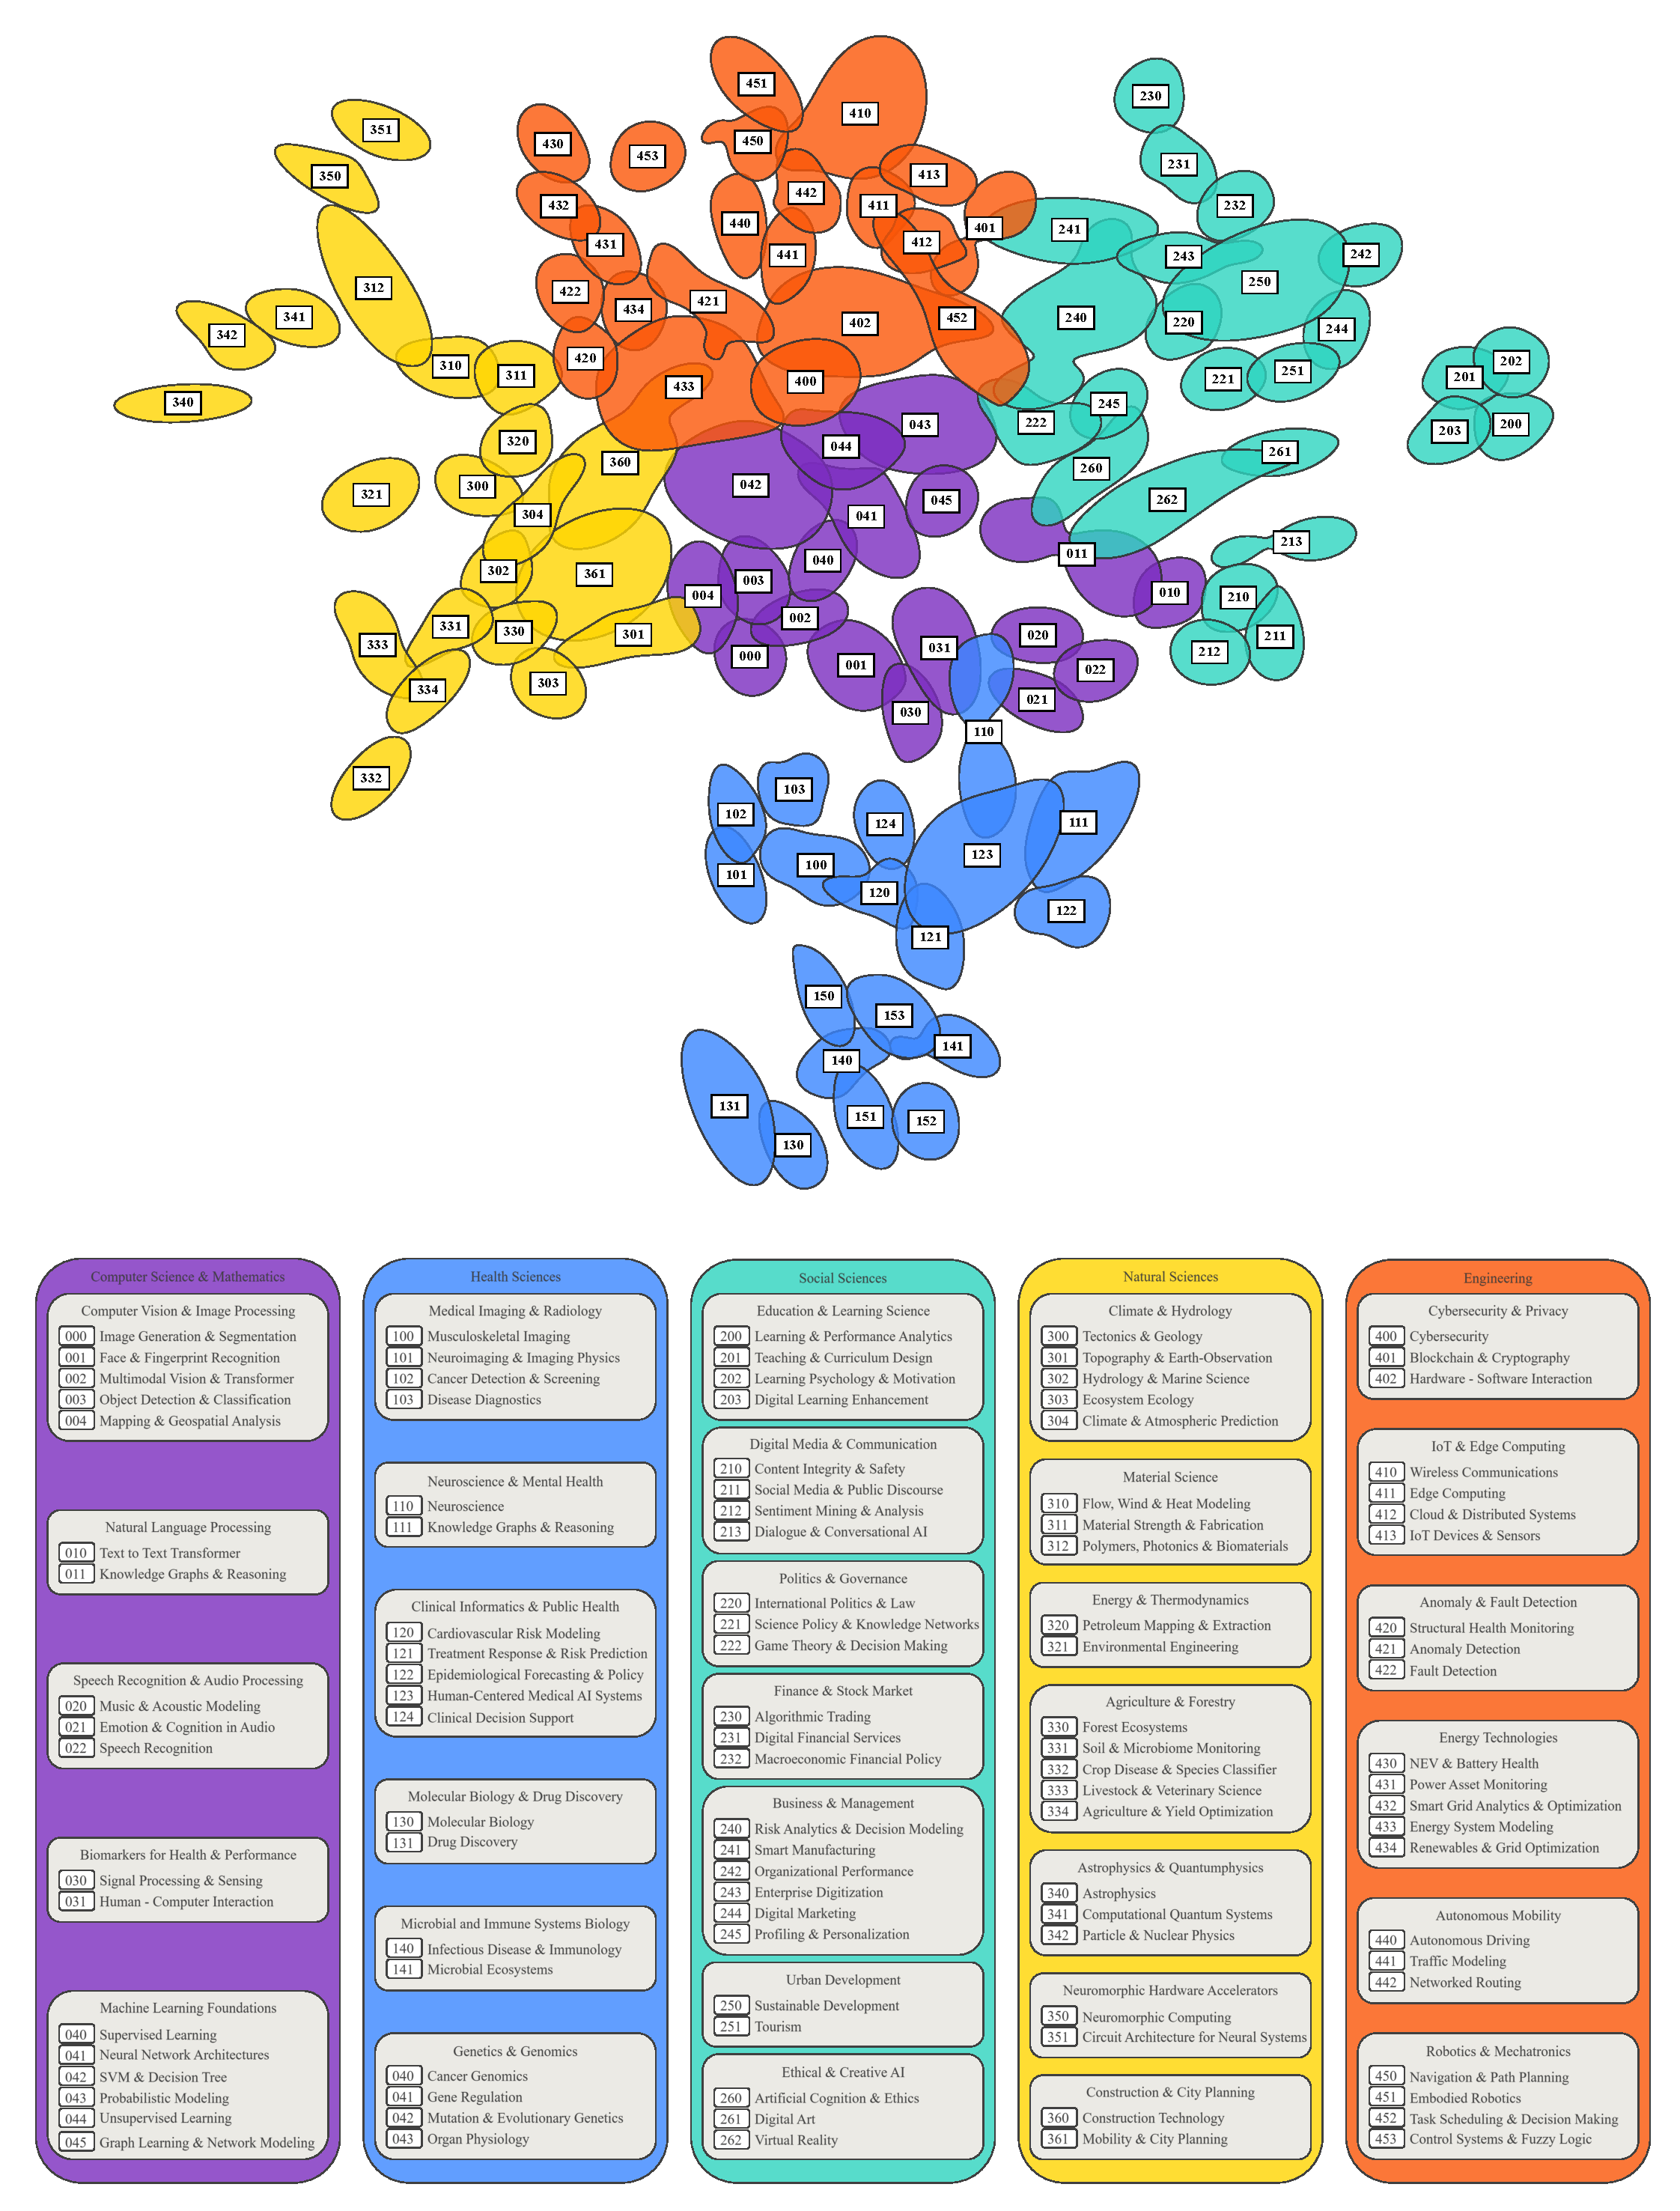
\includegraphics[width=\linewidth]{cluster_umap_with_legend_2025_10_09_bigger_clusters.pdf}
			\vspace{1em}
			\caption*{\small\textit{Density-summarized UMAP of the 106 micro-clusters identified in the SPECTER embedding space. Cluster sizes represent semantic spread, not publication volume. The legend displays the full taxonomy of expert-consolidated clusters across the three hierarchies.}}
		\end{center}
	}]
	
	\paragraph{External Validation via Document Intrusion.}
	\label{intrusion_validation}
	
	To test whether the clusters capture coherent semantic units rather than analytical artifacts, the taxonomy was validated with an intrusion-detection protocol adapted from the ``reading tea leaves'' paradigm \cite{chang2009reading}. In each trial a large language model (DeepSeek v4 Flash Thinking) is shown a panel of genuine member documents from a target cluster together with one intruder drawn from another cluster at the same level, and must identify the intruder; a coherent cluster makes the intruder conspicuous. The protocol was run for 1,000 trials per hierarchy level, and detection accuracy is the share of correctly identified intruders.
	
	Accuracy rises as the clustering becomes finer: 46.0\% at the macro-level (h1), 75.0\% at the meso-level (h2), and over 84.0\% at the micro-level (h3), all well above the random-guess baseline. This gradient is expected: intrusion detection depends on the ratio of within-cluster spread to between-cluster separation, and broad macro-domains are internally heterogeneous by construction --- \textbf{\texttt{Computer Science}} \microC{0}, for instance, spans computer vision, natural language processing, and graph learning --- so an intruder is less conspicuous there than among narrow, lexically distinctive micro-clusters. The results thus indicate a hierarchy that is coherent at every level, with separability increasing toward the finer granularities the analysis relies on most.
	
	\subsection{Subdiscipline Citation Shares}
	
	At the entity level, each bloc's share of the fractional citation sum is computed within every cluster of the taxonomy (Figure~\ref{fig:topic_modeling_heatmap}). To limit redundancy, shares are reported at the macro-level and then only for clusters that diverge from their parent; full cluster-level tables are provided in the Supplementary Information.
	
	\textbf{China} (24.1\% of global citations) concentrates its lead in \textbf{\texttt{Computer Science}} \microC{0} (32.8\%) and \textbf{\texttt{Engineering}} \microE{4} (30.0\%), holds a thin lead in \textbf{\texttt{Natural Science}} \microN{3} (23.6\% vs the EU-27's 23.4\%), and trails in \textbf{\texttt{Health Science}} \microH{1} (18.3\%) and \textbf{\texttt{Social Science}} \microS{2} (13.8\%). It leads 17 of 31 meso- and 44 of 106 micro-clusters, exceeding 40\% thirteen times, with peaks in \textbf{\texttt{Fault Detection}} \microE{422} (57.3\%), \textbf{\texttt{Control Systems \& Fuzzy Logic}} \microE{453} (52.2\%), and \textbf{\texttt{Object Detection \& Classification}} \microC{003} (48.9\%). Its blind spots are equally sharp: \textbf{\texttt{Politics \& Governance}} \microS{22} (5.6\%), \textbf{\texttt{Ethical \& Creative AI}} \microS{26} (6.5\%), and \textbf{\texttt{Astrophysics \& Quantum Physics}} \microN{34} (7.4\%). This discontinuity yields the highest cross-subdiscipline standard deviation of the three blocs (11.77\%).
	
	\textbf{The US} (18.60\%) leads \textbf{\texttt{Health Science}} \microH{1} (23.36\%), ranks second in \textbf{\texttt{Computer Science}} \microC{0} (19.38\%) and \textbf{\texttt{Social Science}} \microS{2} (15.56\%), and last among the blocs in \textbf{\texttt{Natural Science}} \microN{3} (16.83\%) and \textbf{\texttt{Engineering}} \microE{4} (13.65\%). Its strengths cluster in legacy fields --- \textbf{\texttt{Natural Language Processing}} \microC{01} (30.10\%), machine learning, neuroscience, probabilistic modeling, and game theory --- while it falls to single digits in 16 micro-clusters and ranks last in 55 of 106.
	
	\textbf{The EU-27} (20.79\%) shows the most comprehensive coverage. It leads \textbf{\texttt{Social Science}} \microS{2} (25.38\%), follows closely in \textbf{\texttt{Health Science}} \microH{1} (22.87\%) and \textbf{\texttt{Natural Science}} \microN{3} (23.45\%), and trails more clearly only in \textbf{\texttt{Computer Science}} \microC{0} (15.28\%) and \textbf{\texttt{Engineering}} \microE{4} (16.83\%). Only four micro-clusters fall below 10\% (against 14 for China and 16 for the US), and its micro-level standard deviation is the lowest (7.02\%, vs the US's 7.94\% and China's 11.77\%). Its one systematic weakness is the visual-data region: \textbf{\texttt{Computer Vision \& Image Processing}} \microC{00} (12.57\%) and related clusters in supervised and graph learning.
	
	The residual \textbf{RoW} category (36.51\%) lacks institutional cohesion but usefully indicates where the blocs are most consolidated. It would lead four of five macro-clusters and 77 of 106 micro-clusters; its lowest shares --- and thus the strongest bloc consolidation --- fall in the resource-intensive \textbf{\texttt{Genetics \& Genomics}} \microH{15} (24.52\%), \textbf{\texttt{Astrophysics \& Quantum Physics}} \microN{34} (27.47\%), and \textbf{\texttt{Robotics \& Mechatronics}} \microE{45} (30.16\%).
	
	\twocolumn[{%
		\begin{center}
			\vspace{-3em}
			\captionof{figure}{Fractional Citation Shares of the Blocs and RoW across Hierarchical AI Subdisciplines}
			\vspace{1em}
			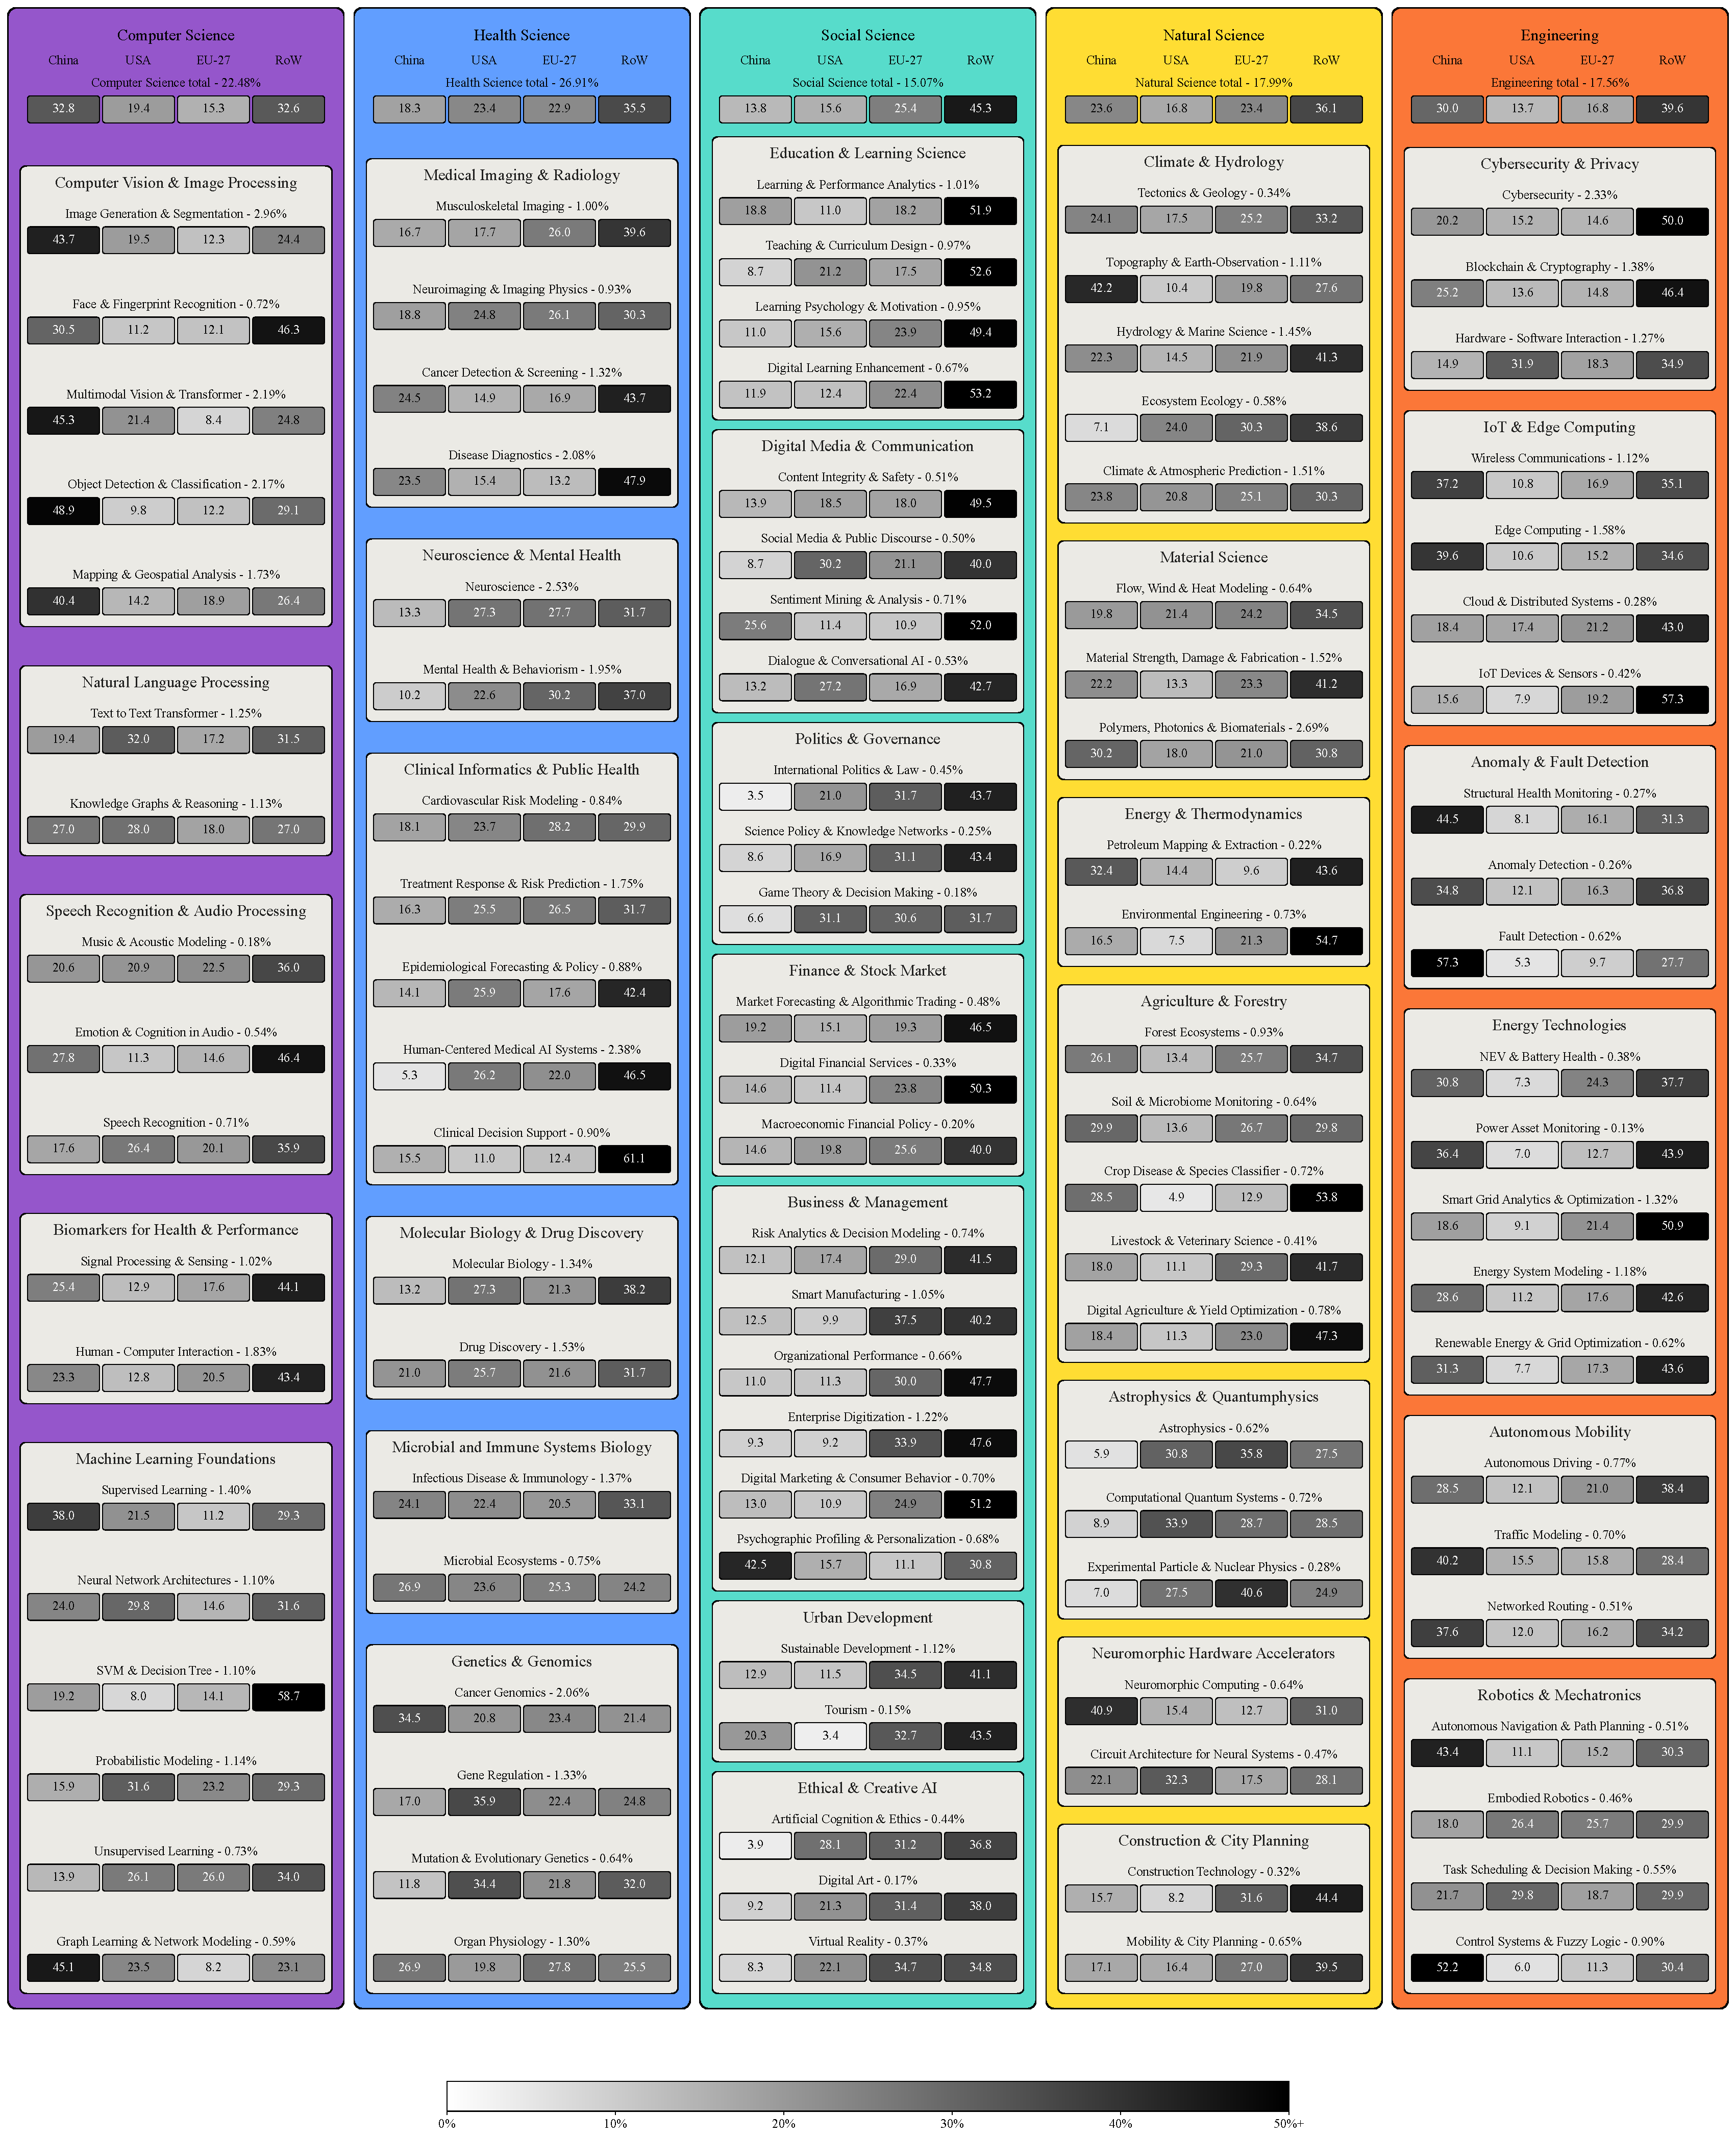
\includegraphics[width=\linewidth]{bloc_citation_shares_across_subdisciplines.pdf}
			\vspace{1em}
			\caption*{\small\textit{Each bloc's share of fractional citation sums across the 106 micro-clusters. Columns correspond to macro-domains, grouped into meso- and micro-clusters by numeric identifier. Mini-heatmaps give the fractional citation shares of the blocs and the residual RoW category; color intensity encodes shares from zero to 50\%.}}
			\label{fig:topic_modeling_heatmap}
			\vspace{2em}
		\end{center}
	}]
	
	\section{Limitations}
	\label{conclusion_limitations}
	
	Several constraints bound the interpretation of these results. \textit{Zero-sum by design:} because citation shares sum to 100\% within each cluster, one bloc's gain is mechanically another's loss; this is a property of the measure and not an endorsement of a realist, zero-sum reading of AI competition. \textit{Scientometric caveats:} citation-based indicators are distorted by goal-setting and evaluation incentives \cite{baccini2019citation, fire2018over}, encode heterogeneous and ambiguous citing functions \cite{adler2009citation, waltman2016review}, reflect visibility and prestige as much as intellectual contribution \cite{waltman2016review}, carry systematic Anglophone and legacy bias \cite{Maddi2025GeographicalDisciplinaryCoverage, gomez2022leading}, and are subject to cumulative advantage \cite{wang2013quantifying, lariviere2009impact}. \textit{Topic modeling:} clusters are interpretive abstractions whose boundaries depend on embedding choice, dimensionality reduction, and random seeds, with errors propagating across the hierarchy (a per-layer precision of 90\% implies roughly 72.9\% reliability over three levels); the document-intrusion validation in Section~\ref{intrusion_validation} mitigates but does not eliminate this concern. \textit{Temporal coverage:} a contemporary corpus offers immediacy at the cost of depth, and with the youngest papers only six months old, citation indicators are informed conjecture rather than settled assessment. No dataset or method is neutral; within these boundaries, the study offers a systematic and transparent approximation of global AI research dynamics.
	
	\section{Conclusion}
	
	This study mapped the global landscape of AI research from 2020 to 2025 and the relative impact of its three leading actors. The key findings are summarized by research question.
	
	\vspace{1em}
	\rule{\linewidth}{0.4pt}
	\begin{enumerate}
		\item[\textbf{RQ1}]\hspace*{2em}\parbox[t]{\dimexpr\linewidth-2em}{
			\textit{Which subdisciplines structure the contemporary AI research landscape?}
		}
	\end{enumerate}
	\vspace{0.25em}
	\rule{\linewidth}{0.4pt}
	\vspace{1em}
	
	The hierarchical topic model subdivided the corpus into 5 domains, 31 fields, and 106 research fronts, with a clear core--periphery structure: a methodological computer-science core --- machine learning, neural networks, computer vision --- encircled by four application domains whose semantic distance from the core grows with their specialization. The document-intrusion validation confirmed coherent clusters at every level (over 84\% detection at the micro-level, 75\% at the meso-level, 46\% at the macro-level), with the lower macro score reflecting the inherent diffuseness of broad domains. This diversity exposes the limits of treating AI as a uniform field and helps explain the wide cross-subdiscipline variation in bloc impact. Two further patterns stand out: research concentrates where commercial application already exists, leaving governance and ethics at just 2.7\% of the corpus despite their public salience; and the periphery outgrows the core (22.15\% overall against 14.74\% for computer science), consistent with AI functioning as a general-purpose technology whose lowest-hanging fruit now lies in fields historically distant from it.
	
	\vspace{1em}
	\rule{\linewidth}{0.4pt}
	\begin{enumerate}
		\item[\textbf{RQ2}]\hspace*{2em}\parbox[t]{\dimexpr\linewidth-2em}{
			\textit{How are the three blocs positioned within these subdisciplines in terms of their relative research impact?}
		}
	\end{enumerate}
	\vspace{0.25em}
	\rule{\linewidth}{0.4pt}
	\vspace{1em}
	
	Across the corpus, China, the EU-27, and the US together account for 58.9\% of publications and 63.5\% of citations. Within the subdisciplines, however, their profiles diverge sharply. The \textbf{EU-27} (20.79\%) is the most balanced: it leads the social sciences, is strong in the health and natural sciences, and has the fewest blind spots --- the lowest cross-subdiscipline standard deviation and only four single-digit micro-clusters. \textbf{China} (24.1\%) holds the largest share but the most focused profile, dominating computer science and engineering --- computer vision, anomaly detection, robotics --- while trailing in the social and health sciences, a high standard deviation that points to strategic specialization. The \textbf{US} (18.60\%) leads in health science and in legacy computer-science fields but ranks last among the blocs in engineering and natural science --- a profile that contrasts sharply with the dominance of its proprietary models and technology firms and underscores how multi-layered AI development is.
	
	These findings also point to further work. Disentangling methodological from domain-specific vocabulary (for example through dual-embedding models) could sharpen the cluster topology; measuring impact through citations attracted from outside an entity's own bloc would reduce intra-system inflation; and the proximity of several Australian and East Asian institutions to the Chinese cluster invites systematic study of how geography, trade, and migration --- beyond cultural and political ties --- predict international collaboration.
	
	\section*{Data and Code}
	
	All code and figures developed for this study are available at \url{https://github.com/Pigeon-Effect/scientometric-analysis-of-ai-research}, covering data retrieval from OpenAlex, topic modeling, citation analysis, and figure generation.
	
	\section*{Declarations}
	
	\textbf{Funding} The authors received no specific funding for this work.
	
	\textbf{Competing interests} The authors declare that they have no competing interests.
	
	
	\section*{Acknowledgements}
	
	The authors thank the OpenAlex team for open access to their API, which enabled the collection of the publication metadata central to this study.
	
	\section*{References}
	
	\printbibliography[heading=none]
	
\end{document}